\documentclass{article}
\usepackage{graphicx}
\usepackage{float}
\usepackage[table]{xcolor}
\usepackage{amsmath}
\usepackage{booktabs}
\usepackage{caption}
\usepackage{subcaption}
\usepackage{geometry}
\usepackage{array}
\usepackage{tabularx}
\usepackage{hyperref}
\usepackage[nottoc,numbib]{tocbibind}
\usepackage[titletoc,toc,page]{appendix}
\addtocontents{toc}{\protect\thispagestyle{empty}}

\geometry{a4paper, margin=1in}
\definecolor{TikTokBlack}{HTML}{040404}
\definecolor{TikTokPink}{HTML}{de8c9d}
\definecolor{TikTokRed}{HTML}{fe2858}
\definecolor{TikTokLightBlue}{HTML}{2af0ea}
\definecolor{TikTokDarkBlue}{HTML}{397684}

\begin{document}

% Center everything on the page
\begin{titlepage}
\begin{center}

    % Logo and title
    
\includegraphics[width=0.1\textwidth]{./resources/logo.png} \\
    \vspace{0.5cm}
    {\Huge \textbf{TikTok-Brain}} \\[0.5cm]
    {\LARGE \textit{Lo-fi Prototyping and Usability Testing}} \\[2cm]

\end{center}

    % Mission Statement
    \noindent
    \textbf{\textcolor{TikTokLightBlue}{\Large Mission Statement}} \\[0.3cm]
    \parbox{\textwidth}{
        \large
        To promote stair safety by leveraging the captivating power of video,
        delivering crucial safety messages in an engaging and distraction-free platform.
        % TikTok-Brain is both a community and competition platform that empowers individuals to take sustainable actions.
    } \\[1cm]

    % Value Proposition
    \noindent
    \textbf{\textcolor{TikTokBlack}{\Large Value Proposition}} \\[0.3cm]
    \parbox{\textwidth}{
        \large
        % Teamwork makes the green work.
        Delivering mesmerizing, randomized videos paired with essential safety advisories,
        TikTok-Brain simplifies social media to focus solely on enhancing personal safety without the clutter of likes, comments, or shares.
    } \\[1cm]


    % Problem / Solution Overview
    \noindent
    \textbf{\textcolor{TikTokRed}{\Large Problem / Solution Overview}} \\[0.3cm]
    \parbox{\textwidth}{
        \large
        Many individuals are unaware of the risks associated with inattentive stair use.
        Traditional safety messages often fail to engage audiences, leading to continued accidents and injuries.
        TikTok-Brain combines the engaging nature of short-form video content with critical safety messaging.
        By removing typical social media distractions,
        the app ensures that users receive and retain important information about walking safely on stairs.
    } \\[1.5cm]

\begin{center}
    % Our Team
    \textbf{\textcolor{TikTokBlack}{\Large Our Team}} \\[0.5cm]

    % Team Photos and Names
    \begin{tabular}{ccc}
        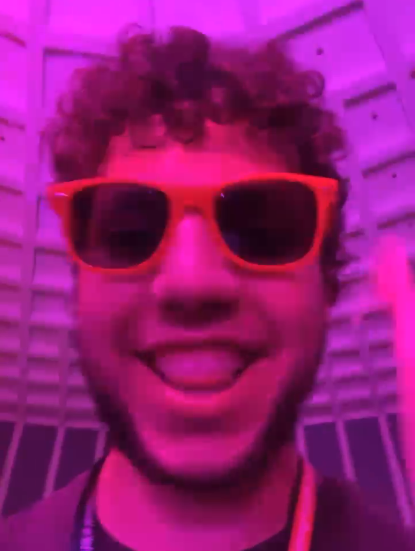
\includegraphics[width=0.2\textwidth]{./resources/ole.png} &
        
\includegraphics[width=0.2\textwidth]{./resources/markus.png} &
        
\includegraphics[width=0.2\textwidth]{./resources/diba.png} \\[0.3cm]
        Ole Einar Grundmann & Markus Siegert & Diba Zokai \\
    \end{tabular}
\end{center}
\end{titlepage}

\newpage
\tableofcontents
\newpage

\section{Introduction}
% Provide an introduction to the project, discussing the background, motivation, and objectives of your work. Describe the problem in more detail and explain why sustainability is crucial.
Distracted walking has become a significant safety concern, particularly on stairs where attention is crucial.
Traditional social media platforms, designed for high engagement,
inadvertently increase these risks by encouraging users to focus more on their screens than their surroundings.

TikTok-Brain is designed to counteract this issue by combining the engaging nature of video content
with crucial safety messages about walking safely on stairs.
This app simplifies the social media model: it removes likes, comments, and shares,
focusing solely on delivering safety-oriented content through mesmerizing, randomized videos paired with safety advisories.

\section{Methodology}
% This section explains the methodology used in your project. Break it down into subsections for clarity.
The process began with an individual brainstorming phase,
where each team member independently generated ideas.
These ideas were then collectively refined using digital tools such as LaTeX, Gimp, and Krita,
resulting in a diverse array of 25 to 30 potential concepts.

To ensure our ideas were aligned with user needs and expectations,
we proceeded to create and conduct a detailed survey comprising 20 questions,
which was administered to 30 participants using Telekom Vote 2 and WhatsApp to reach out to the participants.
The results helped constructing personas and refine our initial ideas.

With a solid understanding of our user base,
we evaluated the brainstormed ideas through a structured pro-contra analysis,
taking into account the feedback and personas developed earlier.
This phase of assessment was supported by Markdown and LaTeX,
allowing us to narrow down our options to three final ideas.

Subsequently, we moved to visually conceptualize these ideas through sketches and storyboards,
utilizing Gimp, other graphic tools, and Kdenlive.
This step was to visualize the sequence and flow of interactions,
which were used for the later stages of prototyping.

In a presentation to gather user feedback,
participants evaluated the top three ideas from each of six groups, totaling 21 ideas.
Each of the 25 attendees had two votes to allocate,
allowing them to identify the concepts they found most compelling.
This iterative process of development and refinement led to the selection
of the most promising prototype based on its functionality and user feedback.

The final stage of our project involved the creation of professional presentations and a comprehensive final report,
crafted using PowerPoint and LaTeX. These documents provided a detailed overview of the project process,
from the initial concept to the final evaluation of the prototype.

\section{Results}
This chapter presents the progression from the already refined concept sketches to the final prototype,
detailing the design decisions, evaluations, and functionality development.

\subsection{Concept Sketches}
The top 3 of our ideas were:

\begin{enumerate}
    \item \textbf{Stair Master:} a versus game where the player has to climb stairs efficiently and safe.
    \item \textbf{StAIr:} an AI image generator where people falling down the stairs with safety prompts embedded.
    \item \textbf{TikTok-Brain:} daily TikTok brainrot bundled inside an application to focus on safety prompts.
\end{enumerate}

\pagebreak

\begin{figure}[H]
    \centering
    \begin{subfigure}[t]{0.45\textwidth}
        \centering
        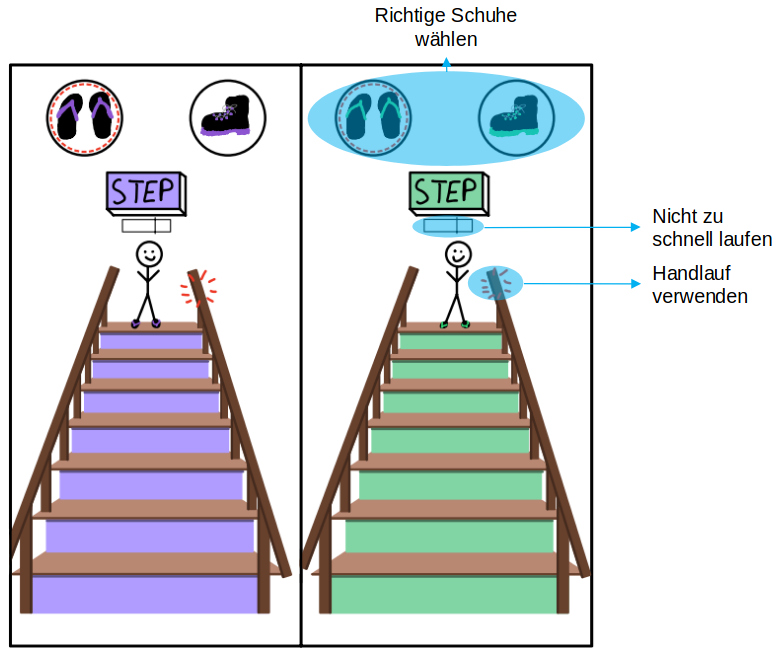
\includegraphics[width=\textwidth]{./resources/StairMaster_1.png}
        \caption{1}
    \end{subfigure}
    \hfill
    \begin{subfigure}[t]{0.45\textwidth}
        \centering
        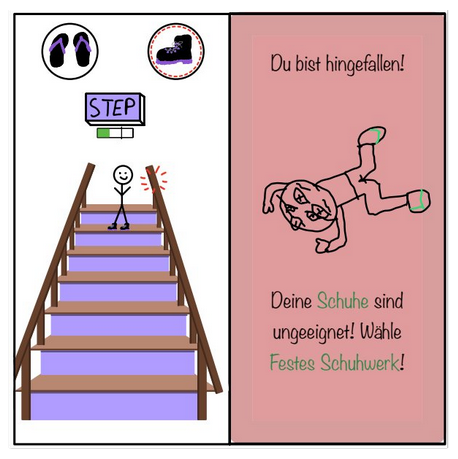
\includegraphics[width=\textwidth]{./resources/StairMaster_2.png}
        \caption{2}
    \end{subfigure}

    \vspace{0.5cm}

    \begin{subfigure}[t]{0.45\textwidth}
        \centering
        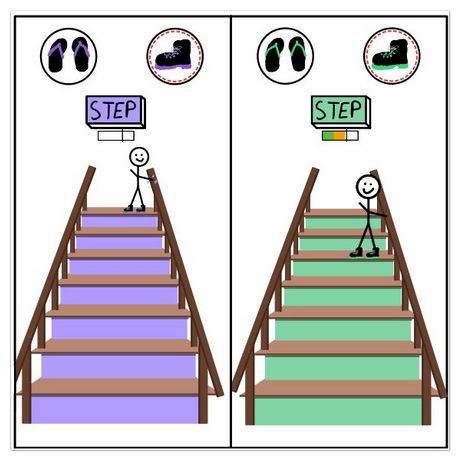
\includegraphics[width=\textwidth]{./resources/StairMaster_3.png}
        \caption{3}
    \end{subfigure}
    \hfill
    \begin{subfigure}[t]{0.45\textwidth}
        \centering
        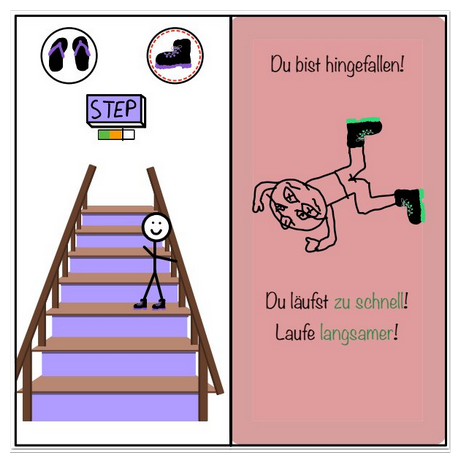
\includegraphics[width=\textwidth]{./resources/StairMaster_4.png}
        \caption{4}
    \end{subfigure}

    \vspace{0.5cm}

    \begin{subfigure}[t]{0.45\textwidth}
        \centering
        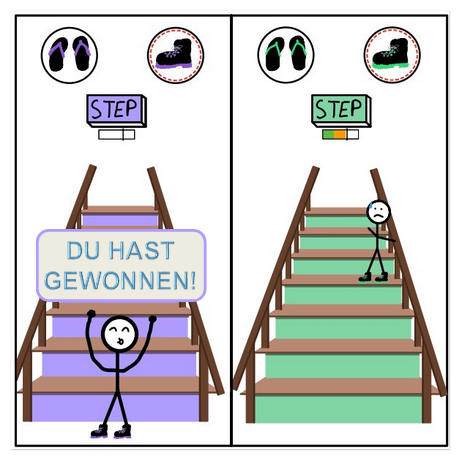
\includegraphics[width=\textwidth]{./resources/StairMaster_5.png}
        \caption{5}
    \end{subfigure}
    \hfill
    \begin{subfigure}[t]{0.45\textwidth}
        \centering
        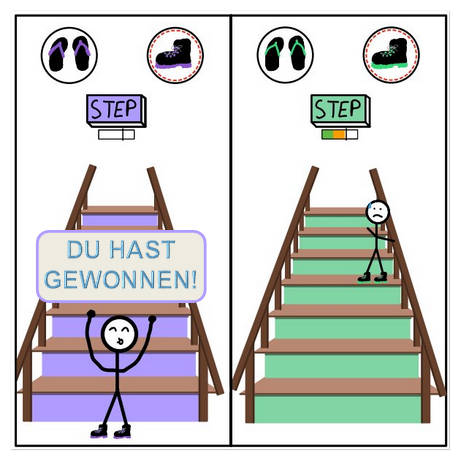
\includegraphics[width=\textwidth]{./resources/StairMaster_6.png}
        \caption{6}
    \end{subfigure}

    \caption{Stair Master Game}
    \label{fig:StairMaster}
\end{figure}

\begin{figure}[H]
    \centering
    \begin{subfigure}[H]{0.8\textwidth}
        \centering
        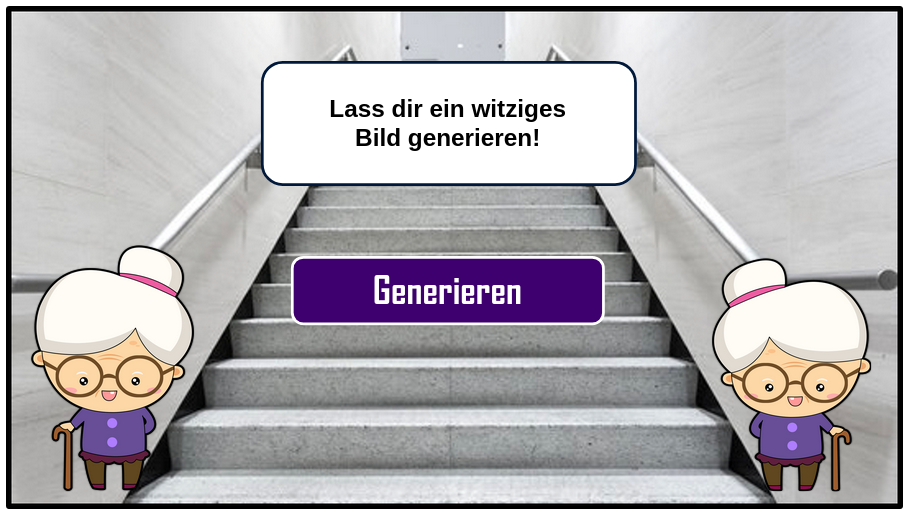
\includegraphics[width=\textwidth]{./resources/StairImgAI_1.png}
        \caption{1}
    \end{subfigure}
    \hfill
    \begin{subfigure}[H]{0.8\textwidth}
        \centering
        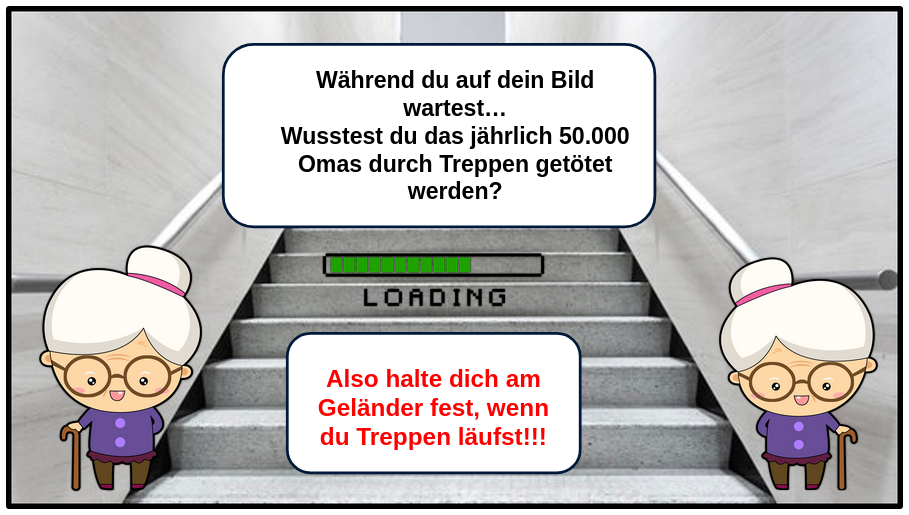
\includegraphics[width=\textwidth]{./resources/StairImgAI_2.png}
        \caption{2}
    \end{subfigure}
    \hfill
    \begin{subfigure}[H]{0.8\textwidth}
        \centering
        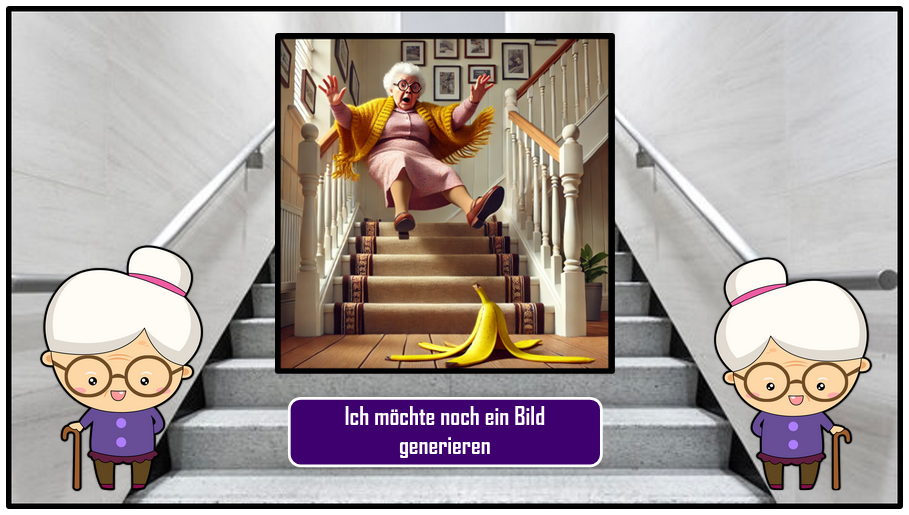
\includegraphics[width=\textwidth]{./resources/StairImgAI_3.png}
        \caption{3}
    \end{subfigure}
    \caption{StAIr AI Image Generation}
    \label{fig:StairImgAI}
\end{figure}

\begin{figure}[H]
    \centering
    \begin{subfigure}[t]{0.45\textwidth}
        \centering
        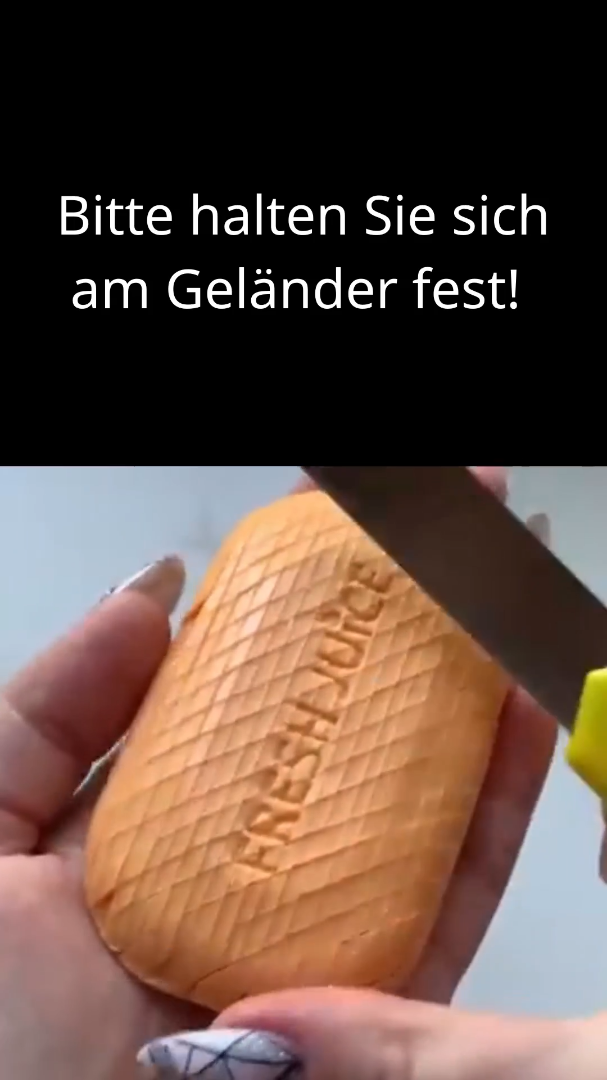
\includegraphics[width=\textwidth]{./resources/StairTikTokBrain_1.png}
        \caption{1}
    \end{subfigure}
    \hfill
    \begin{subfigure}[t]{0.45\textwidth}
        \centering
        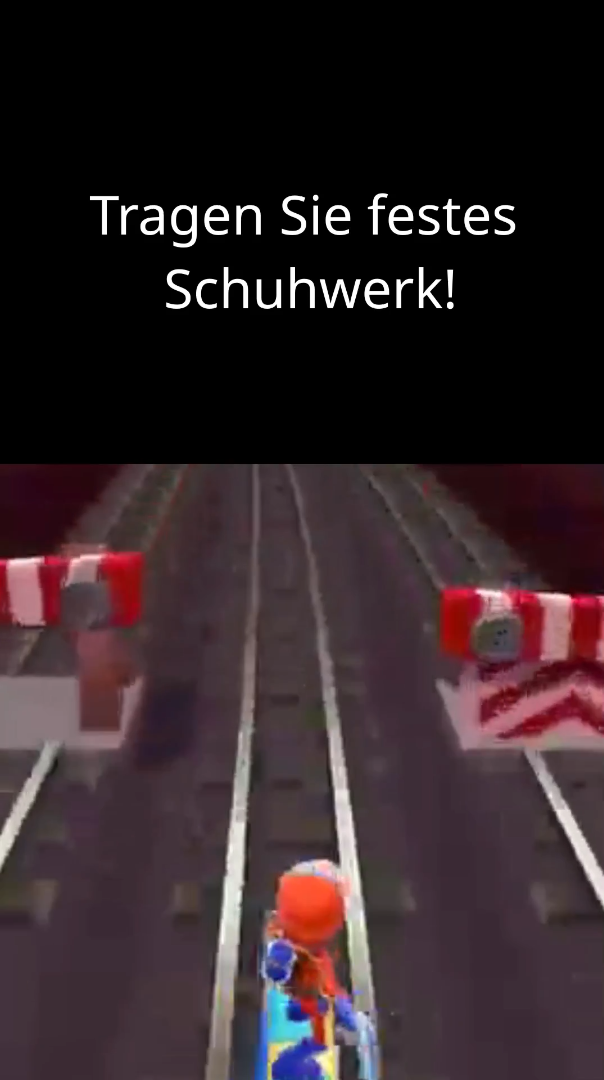
\includegraphics[width=\textwidth]{./resources/StairTikTokBrain_2.png}
        \caption{2}
    \end{subfigure}
    \caption{TikTok-Brain}
    \label{fig:StairTikTokBrain}
\end{figure}


\subsection{Selected Interface Designs}


\begin{table}[H]
\centering
    \textbf{\textcolor{TikTokBlack}{\large Stair Master Game (1 vote)\strut}}\par
\renewcommand{\arraystretch}{1.5}
\setlength{\tabcolsep}{12pt}
    \begin{tabularx}{\textwidth}{|>{\centering\arraybackslash}X|>{\centering\arraybackslash}X|}
\hline
    \cellcolor{TikTokRed}\textbf{Pros} & \cellcolor{TikTokLightBlue}\textbf{Cons} \\
        \hline
        \begin{itemize}
            \item The majority enjoys playing minigames
            \item Social Gaming Interest
            \item Gaming Engagement
        \end{itemize} &
        \begin{itemize}
            \item Does not catch much interest
            \item Few positiv feedback
        \end{itemize}
        \\
        \hline
\end{tabularx}
\caption{Pro + Con analysis for rewards interface}
\end{table}


\begin{table}[H]
\centering
    \textbf{\textcolor{TikTokBlack}{\large StAIr AI Image Generator (2 vote)\strut}}\par
\renewcommand{\arraystretch}{1.5}
\setlength{\tabcolsep}{12pt}
    \begin{tabularx}{\textwidth}{|>{\centering\arraybackslash}X|>{\centering\arraybackslash}X|}
\hline
    \cellcolor{TikTokRed}\textbf{Pros} & \cellcolor{TikTokLightBlue}\textbf{Cons} \\
        \hline
        \begin{itemize}
            \item Humor Preference
            \item Catches attention because of AI use
            \item Simple User-Interface
        \end{itemize} &
        \begin{itemize}
            \item Humor is subjective
            \item Potential Insensitivity
            \item Attention may only focus on AI
        \end{itemize}
        \\
        \hline
\end{tabularx}
\caption{Pro + Con analysis for rewards interface}
\end{table}

\begin{table}[H]
\centering
    \textbf{\textcolor{TikTokBlack}{\large Stair TikTok-Brain (11 votes)\strut}}\par
\renewcommand{\arraystretch}{1.5}
\setlength{\tabcolsep}{12pt}
    \begin{tabularx}{\textwidth}{|>{\centering\arraybackslash}X|>{\centering\arraybackslash}X|}
\hline
    \cellcolor{TikTokRed}\textbf{Pros} & \cellcolor{TikTokLightBlue}\textbf{Cons} \\
        \hline
        \begin{itemize}
            \item High Engagement with Memes and Humor
            \item Everyone spends time on short-form streamer daily
            \item Clear Warning Placement
        \end{itemize} &
        \begin{itemize}
            \item Lower Engagement with Short-form Video
            \item Attention may only focus on videos
        \end{itemize}
        \\
        \hline
\end{tabularx}
\caption{Pro + Con analysis for rewards interface}
\end{table}

\begin{figure}[H]
    \centering
    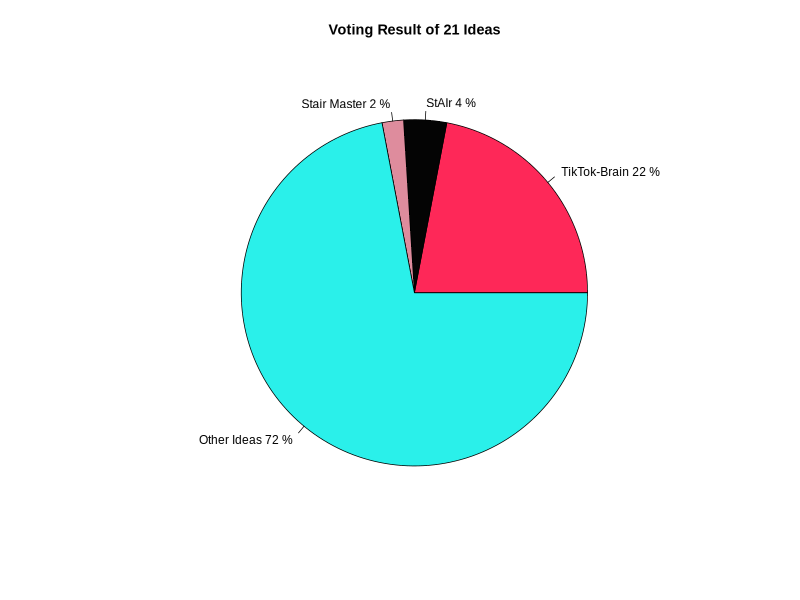
\includegraphics[width=\textwidth]{./ideas_distribution.png}
    \caption{Presentation Voting Results}
    \label{fig:system-overview}
\end{figure}

\subsection{Prototyping}

\begin{figure}[H]
    \centering
    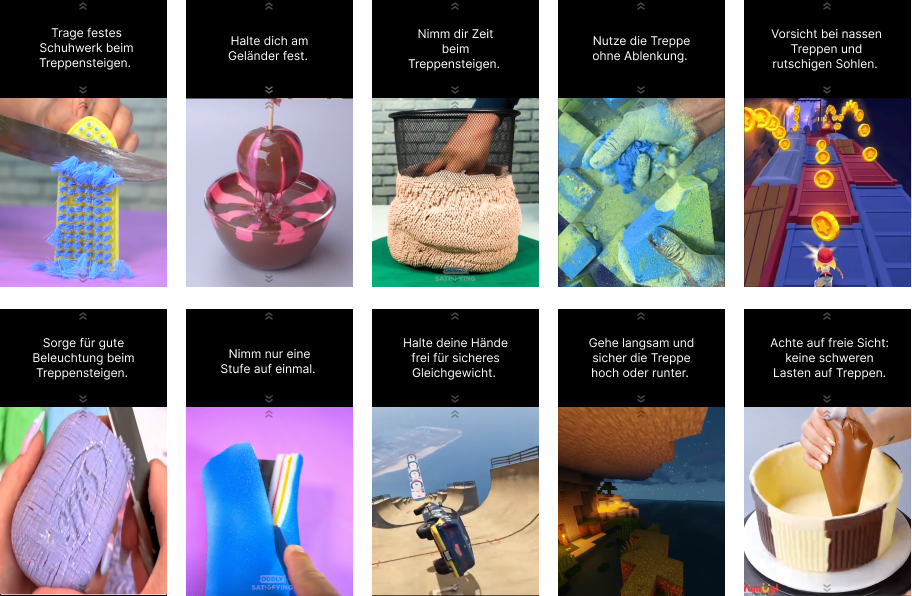
\includegraphics[width=\textwidth]{./resources/storyboard.png}
    \caption{Lo-fi Prototype of TikTok-Brain Platform Interactions}
    \label{fig:storyboard}
\end{figure}

\begin{figure}[H]
    \centering
    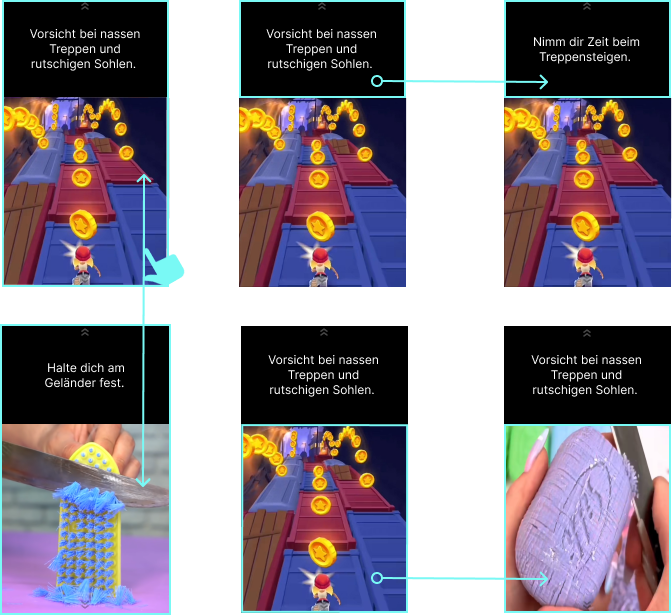
\includegraphics[width=\textwidth]{./resources/full-system.png}
    \caption{Lo-fi Prototype of TikTok-Brain Platform Example Views}
    \label{fig:system-overview}
\end{figure}

\begin{table}[H]
\centering
\renewcommand{\arraystretch}{1.5}
\setlength{\tabcolsep}{12pt}
    \begin{tabularx}{\textwidth}{|l|X|X|}
        \hline
        \cellcolor{TikTokRed}\textbf{Component} & \cellcolor{TikTokBlack}\textbf{\textcolor{white}{Description}} & \cellcolor{TikTokLightBlue}\textbf{Functionality} \\
        \hline
        Video Display Area & Fullscreen area to show videos. & Displays a single video at a time, taking up the bottom part of the screen. \\
        \hline
        Swipe Navigation & Gesture-based navigation for moving through videos. & Swiping up loads the next video; swiping down loads the previous video. \\
        \hline
        Random Video Loader & Logic that fetches a random video to display. & Randomly selects and loads a video from the video pool whenever a new video is required. \\
        \hline
        Text Overlay Area & Area at the top of the screen for text that accompanies each video. & Displays a random line of text (e.g., a phrase or quote) that’s paired with the video. \\
        \hline
        Video-Text Randomizer & Logic that pairs random videos with random text. & Ensures that each video is matched with a different text overlay each time it appears, maintaining freshness. \\
        \hline
        Interface Background & Background color or visual design behind the video display. & Provides visual consistency or mood but stays unobtrusive to keep focus on video and text content. \\
        \hline
        Loading Indicator & Small icon or animation that shows when new content is being loaded. & Briefly appears when the app fetches a new random video or reloads the feed. \\
        \hline
        No Interaction Buttons & No buttons for like, comment, or share, emphasizing simplicity. & Only swipe gestures are recognized; no additional UI elements for social interactions. \\
        \hline
        Error Handling Display & Fallback message or visual when loading fails. & Displays an error message if a video fails to load, with a prompt to restart the application. \\
        \hline
        Auto Swipe Animation & Animation that mimics a swipe if there’s no interaction for a while. & After a set period of inactivity, automatically performs a swipe animation to move to the next video, keeping the experience engaging. \\
        \hline
    \end{tabularx}
    \caption{Functionality of Design Interface Components}
\end{table}

\section{Discussion}
% Analyze the results here, discussing what the results imply about the effectiveness of your platform. Discuss any limitations or challenges encountered.

This chapter discusses these findings in the context of design decisions,
user feedback, usability testing, and future considerations.
Through a structured pro-con analysis, it was evident that an app using short-form video could achieve high engagement,
especially among users already accustomed to similar social media platforms.
However, feedback also highlighted a challenge: while the video format was engaging,
users might still lose interest over time if the content did not vary or if the purpose of the app wasn’t clear.
This feedback led us to focus on creating a highly dynamic and visually engaging app experience.

User feedback was central to the evolution of the TikTok-Brain app.
In the early stages, a pool of 30 participants provided input through surveys,
which helped us understand user preferences and expectations.
Insights from these surveys guided initial design decisions,
including the importance of a distraction-free interface and the appeal of humorous, engaging content.

The pro-con analysis further emphasized the importance of simplicity in the app design.
Through iterative design cycles, the app was refined to eliminate traditional social media features (likes, comments, shares).
This iterative process helped ensure that TikTok-Brain met user expectations,
balanced engagement with educational content, and avoided the pitfalls of over-complicating the interface.

One of the critical design choices in TikTok-Brain was its simplified user interface.
Navigation within the app relied solely on intuitive swipe gestures,
which allowed users to seamlessly move between videos without unnecessary interaction.
This minimalism ensured that safety messages remained the focus point.

While TikTok-Brain successfully demonstrated the potential of short-form video for safety messaging, some limitations were noted.
One limitation is the app’s reliance on randomized video content, which, while engaging,
may not always align with the specific needs or preferences of each user.
Future iterations could incorporate AI-driven personalization to adapt the content based on user interaction patterns,
enhancing the relevance and impact of safety messages.

\section{Conclusion}
% Summarize the key findings and discuss the impact of your work. Outline potential future work or improvements for the platform.
The TikTok-Brain project successfully demonstrates an innovative approach
to delivering safety messages by harnessing the engaging power of short-form video.
Through iterative design and user feedback, we refined the app to ensure it was both intuitive and effective.
The minimalist, swipe-based interface encourages users to focus on the content,
enhancing message retention without the lure of likes, comments, or other interactive elements.

While the randomized video approach proved engaging,
future iterations could benefit from personalized content driven by AI,
tailoring safety messages more closely to user behaviors and preferences.
Overall, TikTok-Brain represents a promising step forward in digital safety interventions,
merging entertainment with crucial safety information to cultivate awareness and prevent distracted stair usage.
This prototype serves as a foundation for further developments in creating engaging yet purposeful social media applications.

% \newpage
% \bibliographystyle{ieeetr}
% \bibliography{Bibliography}
% \newpage

% \renewcommand{\thesection}{\Alph{section}}

% \appendix

% \section{AI Appendix}
% asdf

\end{document}
